\chapter{Monte Carlo Simulation}\label{introduction-to-python---lesson-8}

\begin{Exercise}[title={(Dice Simulation)}]
Using the function \texttt{randint} of the module \texttt{random} make a
Monte Carlo simulation of rolling three dices to check the probability
of getting the same values on the three of them.

From the probability theory you should expect:

\[P_{d1=d2=d3} = \frac{1}{6}\cdot\frac{1}{6}\cdot\frac{1}{6}\cdot 6 = \frac{1}{36} = 0.0278\]
\end{Exercise}
\begin{Answer}
\begin{tcolorbox}[size=fbox, boxrule=1pt, colback=cellbackground, colframe=cellborder]
\begin{Verbatim}[commandchars=\\\{\}]
\PY{k+kn}{from} \PY{n+nn}{random} \PY{k}{import} \PY{n}{seed}\PY{p}{,} \PY{n}{randint}
        
\PY{n}{seed}\PY{p}{(}\PY{l+m+mi}{1}\PY{p}{)}
        
\PY{n}{trials} \PY{o}{=} \PY{l+m+mi}{10000000}
\PY{n}{success} \PY{o}{=} \PY{l+m+mi}{0}
\PY{k}{for} \PY{n}{\PYZus{}} \PY{o+ow}{in} \PY{n+nb}{range}\PY{p}{(}\PY{n}{trials}\PY{p}{)}\PY{p}{:}{6}\PY{p}{)}\PY{p}{,} \PY{n}{randint}\PY{p}{(}\PY{l+m+mi}{1}\PY{p}{,} \PY{l+m+mi}{6}\PY{p}{)}\PY{p}{,} \PY{n}{randint}\PY{p}{(}\PY{l+m+mi}{1}\PY{p}{,} \PY{l+m+mi}{6}\PY{p}{)}    
    \PY{k}{if} \PY{n}{d1} \PY{o}{==} \PY{n}{d2} \PY{o+ow}{and} \PY{n}{d2} \PY{o}{==} \PY{n}{d3}\PY{p}{:}
        \PY{n}{success} \PY{o}{+}\PY{o}{=} \PY{l+m+mi}{1}
    
\PY{n+nb}{print} \PY{p}{(}\PY{l+s+s2}{\PYZdq{}}\PY{l+s+s2}{The probability to get three equal dice is }\PY{l+s+si}{\PYZob{}:.4f\PYZcb{}}\PY{l+s+s2}{\PYZdq{}}\PY{o}{.}\PY{n}{format}\PY{p}{(}\PY{n}{success}\PY{o}{/}\PY{n}{trials}\PY{p}{)}\PY{p}{)}
        
The probability to get three equal dice is 0.0278
\end{Verbatim}
\end{tcolorbox}
\end{Answer}

\begin{Exercise}[title={(Dice simulation II)}]
Two fair dice are rolled, find the probability that their sum is:
\begin{enumerate}
	\item equal to 1
	\item equal to 4
	\item less than 13
\end{enumerate}
	
\textbf{Hint:} the possible combinations of the outcomes of two dice are 36 (to realize it you can simply think that for each one of the six faces of the first die you have six possible faces of the second hence $6\cdot 6=36$). It is not possible to get 1 since 	the dice have no face with 0 so the first probability should come out 0. The sum of the two dice is always less than 13 (the maximum is 12\ldots) so the answer to point 3 is 1. We can get a sum of 4 in 3 cases (1-3, 3-1 or 2-2) so the expected probability is $3/36=1/12=0.0833$
\end{Exercise}

\begin{Answer}
\begin{tcolorbox}[breakable, size=fbox, boxrule=1pt, pad at break*=1mm,colback=cellbackground, colframe=cellborder]
\begin{Verbatim}[commandchars=\\\{\}]
\PY{k+kn}{import} \PY{n+nn}{random}
	
\PY{n}{random}\PY{o}{.}\PY{n}{seed}\PY{p}{(}\PY{l+m+mi}{1}\PY{p}{)}
	
\PY{n}{successes} \PY{o}{=} \PY{p}{\PYZob{}}\PY{l+s+s2}{\PYZdq{}}\PY{l+s+s2}{=0}\PY{l+s+s2}{\PYZdq{}}\PY{p}{:}\PY{l+m+mf}{0.0}\PY{p}{,} \PY{l+s+s2}{\PYZdq{}}\PY{l+s+s2}{=4}\PY{l+s+s2}{\PYZdq{}}\PY{p}{:}\PY{l+m+mf}{0.0}\PY{p}{,} \PY{l+s+s2}{\PYZdq{}}\PY{l+s+s2}{\PYZlt{}13}\PY{l+s+s2}{\PYZdq{}}\PY{p}{:}\PY{l+m+mf}{0.0}\PY{p}{\PYZcb{}}
\PY{n}{trials} \PY{o}{=} \PY{l+m+mi}{100000}
\PY{k}{for} \PY{n}{\PYZus{}} \PY{o+ow}{in} \PY{n+nb}{range}\PY{p}{(}\PY{n}{trials}\PY{p}{)}\PY{p}{:}
    \PY{n}{d1} \PY{o}{=} \PY{n}{random}\PY{o}{.}\PY{n}{randint}\PY{p}{(}\PY{l+m+mi}{1}\PY{p}{,} \PY{l+m+mi}{6}\PY{p}{)}
    \PY{n}{d2} \PY{o}{=} \PY{n}{random}\PY{o}{.}\PY{n}{randint}\PY{p}{(}\PY{l+m+mi}{1}\PY{p}{,} \PY{l+m+mi}{6}\PY{p}{)}
    \PY{k}{if} \PY{p}{(}\PY{n}{d1} \PY{o}{+} \PY{n}{d2}\PY{p}{)} \PY{o}{==} \PY{l+m+mi}{0}\PY{p}{:}
        \PY{n}{successes}\PY{p}{[}\PY{l+s+s2}{\PYZdq{}}\PY{l+s+s2}{=0}\PY{l+s+s2}{\PYZdq{}}\PY{p}{]} \PY{o}{+}\PY{o}{=} \PY{l+m+mf}{1.0}
    \PY{k}{if} \PY{p}{(}\PY{n}{d1} \PY{o}{+} \PY{n}{d2}\PY{p}{)} \PY{o}{==} \PY{l+m+mi}{4}\PY{p}{:}
        \PY{n}{successes}\PY{p}{[}\PY{l+s+s2}{\PYZdq{}}\PY{l+s+s2}{=4}\PY{l+s+s2}{\PYZdq{}}\PY{p}{]} \PY{o}{+}\PY{o}{=} \PY{l+m+mf}{1.0}
    \PY{k}{if} \PY{p}{(}\PY{n}{d1} \PY{o}{+} \PY{n}{d2}\PY{p}{)} \PY{o}{\PYZlt{}} \PY{l+m+mi}{13}\PY{p}{:}
        \PY{n}{successes}\PY{p}{[}\PY{l+s+s2}{\PYZdq{}}\PY{l+s+s2}{\PYZlt{}13}\PY{l+s+s2}{\PYZdq{}}\PY{p}{]} \PY{o}{+}\PY{o}{=} \PY{l+m+mf}{1.0}
	
\PY{k}{for} \PY{n}{k}\PY{p}{,}\PY{n}{v} \PY{o+ow}{in} \PY{n}{successes}\PY{o}{.}\PY{n}{items}\PY{p}{(}\PY{p}{)}\PY{p}{:}
    \PY{n+nb}{print} \PY{p}{(}\PY{l+s+s2}{\PYZdq{}}\PY{l+s+s2}{P(}\PY{l+s+si}{\PYZob{}\PYZcb{}}\PY{l+s+s2}{): }\PY{l+s+si}{\PYZob{}:.3f\PYZcb{}}\PY{l+s+s2}{\PYZdq{}}\PY{o}{.}\PY{n}{format}\PY{p}{(}\PY{n}{k}\PY{p}{,} \PY{n}{v}\PY{o}{/}\PY{n}{trials}\PY{p}{)}\PY{p}{)}
	
P(=0): 0.000
P(=4): 0.084
P(<13): 1.000
\end{Verbatim}
\end{tcolorbox}
\end{Answer}



\begin{Exercise}[title={(Monte Carlo Simulation}]
There are 60 chemical flasks in the laboratory, 6 of which are incorrectly labeled. What is the chance that if we randomly choose 5 flasks, exactly 3 of them will be labeled correctly ?

\textbf{Hint:} the probability is approximately 6.8 \%.
\end{Exercise}

\begin{Answer}
\begin{tcolorbox}[breakable, size=fbox, boxrule=1pt, pad at break*=1mm,colback=cellbackground, colframe=cellborder]
\begin{Verbatim}[commandchars=\\\{\}]
\PY{k+kn}{import} \PY{n+nn}{random}

\PY{n}{flasks} \PY{o}{=} \PY{p}{[}\PY{l+s+s2}{\PYZdq{}}\PY{l+s+s2}{C}\PY{l+s+s2}{\PYZdq{}}\PY{p}{]}\PY{o}{*}\PY{l+m+mi}{54} \PY{o}{+} \PY{p}{[}\PY{l+s+s2}{\PYZdq{}}\PY{l+s+s2}{U}\PY{l+s+s2}{\PYZdq{}}\PY{p}{]} \PY{o}{*} \PY{l+m+mi}{6}

\PY{n}{random}\PY{o}{.}\PY{n}{seed}\PY{p}{(}\PY{l+m+mi}{1}\PY{p}{)}
\PY{n}{trials} \PY{o}{=} \PY{l+m+mi}{1000}
\PY{n}{success} \PY{o}{=} \PY{l+m+mf}{0.}
\PY{k}{for} \PY{n}{\PYZus{}} \PY{o+ow}{in} \PY{n+nb}{range}\PY{p}{(}\PY{n}{trials}\PY{p}{)}\PY{p}{:}
    \PY{n}{draw} \PY{o}{=} \PY{n}{random}\PY{o}{.}\PY{n}{sample}\PY{p}{(}\PY{n}{flasks}\PY{p}{,} \PY{l+m+mi}{5}\PY{p}{)}
    \PY{k}{if} \PY{n}{draw}\PY{o}{.}\PY{n}{count}\PY{p}{(}\PY{l+s+s2}{\PYZdq{}}\PY{l+s+s2}{C}\PY{l+s+s2}{\PYZdq{}}\PY{p}{)} \PY{o}{==} \PY{l+m+mi}{3}\PY{p}{:}
        \PY{n}{success} \PY{o}{+}\PY{o}{=} \PY{l+m+mf}{1.}
        
\PY{n+nb}{print} \PY{p}{(}\PY{l+s+s2}{\PYZdq{}}\PY{l+s+s2}{Probbility: }\PY{l+s+si}{\PYZob{}:.1f\PYZcb{}}\PY{l+s+s2}{\PYZpc{}}\PY{l+s+s2}{\PYZdq{}}\PY{o}{.}\PY{n}{format}\PY{p}{(}\PY{n}{success}\PY{o}{/}\PY{n+nb}{float}\PY{p}{(}\PY{n}{trials}\PY{p}{)}\PY{o}{*}\PY{l+m+mi}{100}\PY{p}{)}\PY{p}{)}

Probbility: 6.7\%
\end{Verbatim}
\end{tcolorbox}
\end{Answer}

\begin{Exercise}[title={(Confidence Interval)}]
Given the following historical series (1895-2020) find average September temperature in US and report the 99\% confidence interval of your measure.

Input (temperatures are in Farenheit degrees):
 \begin{Shaded}
\begin{Highlighting}[]
\NormalTok{temperatures }\OperatorTok{=}\NormalTok{[}\FloatTok{65.98}\NormalTok{, }\FloatTok{68.43}\NormalTok{, }\FloatTok{67.53}\NormalTok{, }\FloatTok{66.27}\NormalTok{, }\FloatTok{67.12}\NormalTok{, }\FloatTok{68.54}\NormalTok{, }\FloatTok{66.20}\NormalTok{, }\FloatTok{66.96}\NormalTok{, }\FloatTok{66.31}\NormalTok{, }\FloatTok{66.09}\NormalTok{, }
\FloatTok{66.49}\NormalTok{, }\FloatTok{66.38}\NormalTok{, }\FloatTok{65.21}\NormalTok{, }\FloatTok{66.43}\NormalTok{, }\FloatTok{63.30}\NormalTok{, }\FloatTok{67.37}\NormalTok{, }\FloatTok{65.66}\NormalTok{, }\FloatTok{64.96}\NormalTok{, }\FloatTok{66.85}\NormalTok{, }\FloatTok{65.70}\NormalTok{, }\FloatTok{65.57}\NormalTok{, }\FloatTok{64.35}\NormalTok{, }
\FloatTok{68.99}\NormalTok{, }\FloatTok{66.42}\NormalTok{, }\FloatTok{63.46}\NormalTok{, }\FloatTok{64.69}\NormalTok{, }\FloatTok{65.55}\NormalTok{, }\FloatTok{63.30}\NormalTok{, }\FloatTok{64.67}\NormalTok{, }\FloatTok{64.90}\NormalTok{, }\FloatTok{67.35}\NormalTok{, }\FloatTok{64.08}\NormalTok{, }\FloatTok{64.60}\NormalTok{, }\FloatTok{65.25}\NormalTok{, }
\FloatTok{63.70}\NormalTok{, }\FloatTok{62.73}\NormalTok{, }\FloatTok{63.14}\NormalTok{, }\FloatTok{65.59}\NormalTok{, }\FloatTok{64.04}\NormalTok{, }\FloatTok{64.92}\NormalTok{, }\FloatTok{66.24}\NormalTok{, }\FloatTok{66.09}\NormalTok{, }\FloatTok{65.84}\NormalTok{, }\FloatTok{65.93}\NormalTok{, }\FloatTok{64.18}\NormalTok{, }\FloatTok{62.89}\NormalTok{, }
\FloatTok{62.31}\NormalTok{, }\FloatTok{64.40}\NormalTok{, }\FloatTok{64.44}\NormalTok{, }\FloatTok{64.33}\NormalTok{, }\FloatTok{64.58}\NormalTok{, }\FloatTok{65.55}\NormalTok{, }\FloatTok{63.90}\NormalTok{, }\FloatTok{64.06}\NormalTok{, }\FloatTok{64.54}\NormalTok{, }\FloatTok{61.77}\NormalTok{, }\FloatTok{63.70}\NormalTok{, }\FloatTok{66.34}\NormalTok{, }
\FloatTok{64.18}\NormalTok{, }\FloatTok{63.41}\NormalTok{, }\FloatTok{66.45}\NormalTok{, }\FloatTok{64.74}\NormalTok{, }\FloatTok{65.43}\NormalTok{, }\FloatTok{64.18}\NormalTok{, }\FloatTok{65.10}\NormalTok{, }\FloatTok{65.88}\NormalTok{, }\FloatTok{66.45}\NormalTok{, }\FloatTok{66.16}\NormalTok{, }\FloatTok{65.89}\NormalTok{, }\FloatTok{64.09}\NormalTok{, }
\FloatTok{63.50}\NormalTok{, }\FloatTok{63.73}\NormalTok{, }\FloatTok{66.07}\NormalTok{, }\FloatTok{66.54}\NormalTok{, }\FloatTok{64.54}\NormalTok{, }\FloatTok{64.99}\NormalTok{, }\FloatTok{65.26}\NormalTok{, }\FloatTok{64.33}\NormalTok{, }\FloatTok{63.66}\NormalTok{, }\FloatTok{64.53}\NormalTok{, }\FloatTok{65.35}\NormalTok{, }\FloatTok{67.37}\NormalTok{, }
\FloatTok{66.63}\NormalTok{, }\FloatTok{65.70}\NormalTok{, }\FloatTok{66.36}\NormalTok{, }\FloatTok{64.80}\NormalTok{, }\FloatTok{63.84}\NormalTok{, }\FloatTok{67.73}\NormalTok{, }\FloatTok{64.69}\NormalTok{, }\FloatTok{68.13}\NormalTok{, }\FloatTok{65.75}\NormalTok{, }\FloatTok{63.41}\NormalTok{, }\FloatTok{63.27}\NormalTok{, }\FloatTok{64.98}\NormalTok{, }
\FloatTok{64.11}\NormalTok{, }\FloatTok{66.67}\NormalTok{, }\FloatTok{62.74}\NormalTok{, }\FloatTok{65.07}\NormalTok{, }\FloatTok{67.28}\NormalTok{, }\FloatTok{66.54}\NormalTok{, }\FloatTok{65.44}\NormalTok{, }\FloatTok{65.64}\NormalTok{, }\FloatTok{61.92}\NormalTok{, }\FloatTok{64.09}\NormalTok{, }\FloatTok{63.50}\NormalTok{, }\FloatTok{64.42}\NormalTok{, }
\FloatTok{64.58}\NormalTok{, }\FloatTok{63.64}\NormalTok{, }\FloatTok{62.73}\NormalTok{, }\FloatTok{66.09}\NormalTok{, }\FloatTok{65.68}\NormalTok{, }\FloatTok{64.40}\NormalTok{, }\FloatTok{65.59}\NormalTok{, }\FloatTok{64.22}\NormalTok{, }\FloatTok{66.25}\NormalTok{, }\FloatTok{65.95}\NormalTok{, }\FloatTok{64.96}\NormalTok{, }\FloatTok{62.73}\NormalTok{, }
\FloatTok{62.76}\NormalTok{, }\FloatTok{63.25}\NormalTok{, }\FloatTok{65.14}\NormalTok{, }\FloatTok{64.80}\NormalTok{, }\FloatTok{65.46}\NormalTok{, }\FloatTok{66.40}\NormalTok{, }\FloatTok{62.94}\NormalTok{, }\FloatTok{65.57}\NormalTok{]}
\end{Highlighting}
\end{Shaded}
\end{Exercise}

\begin{Answer}
\begin{tcolorbox}[breakable, size=fbox, boxrule=1pt, pad at break*=1mm,colback=cellbackground, colframe=cellborder]
\begin{Verbatim}[commandchars=\\\{\}]
\PY{k+kn}{from} \PY{n+nn}{scipy}\PY{n+nn}{.}\PY{n+nn}{stats} \PY{k}{import} \PY{n}{norm}
\PY{k+kn}{import} \PY{n+nn}{numpy} \PY{k}{as} \PY{n+nn}{np}
\PY{n}{temperatures} \PY{o}{=}\PY{p}{[}\PY{l+m+mf}{65.98}\PY{p}{,} \PY{l+m+mf}{68.43}\PY{p}{...}\PY{p}{]}
\PY{n}{temperatures} \PY{o}{=} \PY{n}{np}\PY{o}{.}\PY{n}{array}\PY{p}{(}\PY{n}{temperatures}\PY{p}{)}

\PY{n}{alpha} \PY{o}{=} \PY{l+m+mf}{0.99}

\PY{n}{A} \PY{o}{=} \PY{n}{norm}\PY{o}{.}\PY{n}{ppf}\PY{p}{(}\PY{p}{(}\PY{l+m+mi}{1} \PY{o}{+} \PY{n}{alpha}\PY{p}{)}\PY{o}{/}\PY{l+m+mi}{2}\PY{p}{)}
\PY{n}{m}\PY{p}{,} \PY{n}{se} \PY{o}{=} \PY{n}{np}\PY{o}{.}\PY{n}{mean}\PY{p}{(}\PY{n}{temperatures}\PY{p}{)}\PY{p}{,} \PY{n}{np}\PY{o}{.}\PY{n}{std}\PY{p}{(}\PY{n}{temperatures}\PY{p}{)}
\PY{n}{h} \PY{o}{=} \PY{n}{A}\PY{o}{*}\PY{n}{se}\PY{o}{/}\PY{n}{np}\PY{o}{.}\PY{n}{sqrt}\PY{p}{(}\PY{n+nb}{len}\PY{p}{(}\PY{n}{temperatures}\PY{p}{)}\PY{p}{)}

\PY{n+nb}{print} \PY{p}{(}\PY{l+s+s2}{\PYZdq{}}\PY{l+s+s2}{Avg temperature in September (US): }\PY{l+s+si}{\PYZob{}\PYZcb{}}\PY{l+s+s2}{\PYZdq{}}\PY{o}{.}\PY{n}{format}\PY{p}{(}\PY{n}{m}\PY{p}{)}\PY{p}{)} 
\PY{n+nb}{print} \PY{p}{(}\PY{l+s+s2}{\PYZdq{}}\PY{l+s+si}{\PYZob{}:.0f\PYZcb{}}\PY{l+s+si}{\PYZpc{} c}\PY{l+s+s2}{onfidence interval: +\PYZhy{} }\PY{l+s+si}{\PYZob{}\PYZcb{}}\PY{l+s+s2}{\PYZdq{}}\PY{o}{.}\PY{n}{format}\PY{p}{(}\PY{n}{alpha}\PY{o}{*}\PY{l+m+mi}{100}\PY{p}{,} \PY{n}{h}\PY{p}{)}\PY{p}{)}

Avg temperature in September (US): 65.10992063492064
99\% confidence interval: +- 0.33013045424273185
\end{Verbatim}
\end{tcolorbox}
\end{Answer}

\begin{Exercise}[title={(Stochastic Process Simulation)}]
Using the function \texttt{normal} of \texttt{numpy.random} simulate the price of a stock which evolves according to a log-normal stochastic process with a daily rate of return \(\mu=0.1\) and a volatility \(\sigma=0.15\) for 30 days.

Also plot the price. Try to play with \(\mu\) and \(\sigma\) to see how the plot changes.
\end{Exercise}
\vfill
\begin{Answer}
\begin{tcolorbox}[size=fbox, boxrule=1pt, colback=cellbackground, colframe=cellborder]
\begin{Verbatim}[commandchars=\\\{\}]
\PY{k+kn}{from} \PY{n+nn}{numpy}\PY{n+nn}{.}\PY{n+nn}{random} \PY{k}{import} \PY{n}{normal}\PY{p}{,} \PY{n}{seed}
\PY{k+kn}{from} \PY{n+nn}{matplotlib} \PY{k}{import} \PY{n}{pyplot} \PY{k}{as} \PY{n}{plt}
\PY{k+kn}{import} \PY{n+nn}{math}
 
\PY{n}{S} \PY{o}{=} \PY{l+m+mi}{100}
\PY{n}{mu} \PY{o}{=} \PY{l+m+mf}{0.1}
\PY{n}{sigma} \PY{o}{=} \PY{l+m+mf}{0.15}
\PY{n}{T} \PY{o}{=} \PY{l+m+mi}{1}
 
\PY{n}{seed}\PY{p}{(}\PY{l+m+mi}{1}\PY{p}{)}
\PY{n}{historical\PYZus{}series} \PY{o}{=} \PY{p}{[}\PY{n}{S}\PY{p}{]}
\PY{k}{for} \PY{n}{i} \PY{o+ow}{in} \PY{n+nb}{range}\PY{p}{(}\PY{l+m+mi}{30}\PY{p}{)}\PY{p}{:}
     \PY{n}{S} \PY{o}{=} \PY{n}{S} \PY{o}{*} \PY{n}{math}\PY{o}{.}\PY{n}{exp}\PY{p}{(}\PY{p}{(}\PY{n}{mu} \PY{o}{\PYZhy{}} \PY{l+m+mf}{0.5} \PY{o}{*} \PY{n}{sigma} \PY{o}{*} \PY{n}{sigma}\PY{p}{)} \PY{o}{*} \PY{n}{T} \PY{o}{+}
                                       \PY{n}{sigma} \PY{o}{*} \PY{n}{math}\PY{o}{.}\PY{n}{sqrt}\PY{p}{(}\PY{n}{T}\PY{p}{)} \PY{o}{*} \PY{n}{normal}\PY{p}{(}\PY{p}{)}\PY{p}{)}
     \PY{n}{historical\PYZus{}series}\PY{o}{.}\PY{n}{append}\PY{p}{(}\PY{n}{S}\PY{p}{)}
     
\PY{n}{plt}\PY{o}{.}\PY{n}{plot}\PY{p}{(}\PY{n+nb}{range}\PY{p}{(}\PY{l+m+mi}{31}\PY{p}{)}\PY{p}{,} \PY{n}{historical\PYZus{}series}\PY{p}{)}
\PY{n}{plt}\PY{o}{.}\PY{n}{xlabel}\PY{p}{(}\PY{l+s+s2}{\PYZdq{}}\PY{l+s+s2}{days}\PY{l+s+s2}{\PYZdq{}}\PY{p}{)}
\PY{n}{plt}\PY{o}{.}\PY{n}{ylabel}\PY{p}{(}\PY{l+s+s2}{\PYZdq{}}\PY{l+s+s2}{Price of stock X}\PY{l+s+s2}{\PYZdq{}}\PY{p}{)}
\PY{n}{plt}\PY{o}{.}\PY{n}{show}\PY{p}{(}\PY{p}{)}
\end{Verbatim}
\end{tcolorbox}

\begin{center}
  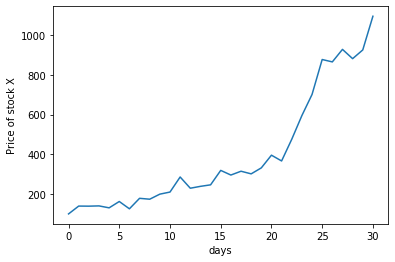
\includegraphics{figures/lesson6_solutions_5_0.png}
\end{center}
\end{Answer}
